\ProvidesFile{themes/japanese-garden/theme.tex}[2026/09/27 Japanese garden poster theme]

\RequirePackage{tgtermes}
\RequirePackage{qrcode}

% ====================
% Theme tokens
% ====================

\definecolor{GardenPaper}{HTML}{F7F0E1}
\definecolor{GardenInk}{HTML}{0F233D}
\definecolor{GardenBlue}{HTML}{168FBE}
\definecolor{GardenMist}{HTML}{BFCED0}
\definecolor{GardenWash}{HTML}{DFE9E6}
\definecolor{GardenRule}{HTML}{607987}
\definecolor{GardenVermilion}{HTML}{C84936}
\definecolor{GardenGray}{HTML}{667078}

\colorlet{CrispWhite}{GardenPaper}
\colorlet{DarkNavy}{GardenInk}
\colorlet{Aqua}{GardenBlue}
\colorlet{SkyBlue}{GardenWash}
\colorlet{TakeawayAccent}{GardenVermilion}
\colorlet{SoftGray}{GardenGray}

\setbeamercolor{normal text}{fg=GardenInk,bg=}
\setbeamercolor{structure}{fg=GardenBlue}
\setbeamercolor{item}{fg=GardenBlue}
\setbeamercolor{headline}{fg=GardenInk,bg=}
\setbeamercolor{headline title}{fg=GardenInk,bg=}
\setbeamercolor{headline author}{fg=GardenInk,bg=}
\setbeamercolor{headline institute}{fg=GardenInk,bg=}
\setbeamercolor{block title}{fg=GardenInk,bg=}
\setbeamercolor{block separator}{bg=GardenRule}
\setbeamercolor{block body}{fg=GardenInk,bg=}
\setbeamercolor{block alerted title}{fg=GardenInk,bg=}
\setbeamercolor{block alerted separator}{bg=GardenRule}
\setbeamercolor{block alerted body}{fg=GardenInk,bg=GardenWash}
\setbeamercolor{caption name}{fg=GardenBlue}
\setbeamercolor{caption}{fg=GardenInk}
\setbeamercolor{garden footer}{fg=GardenInk,bg=}
\setbeamercolor{garden footer rule}{bg=GardenRule}

\usefonttheme{serif}
\setbeamerfont{normal text}{family=\rmfamily,size=\large}
\setbeamerfont{headline title}{family=\rmfamily,size=\Huge,series=\bfseries}
\setbeamerfont{headline author}{family=\rmfamily,size=\Large}
\setbeamerfont{headline institute}{family=\rmfamily,size=\large}
\setbeamerfont{block title}{family=\rmfamily,size=\Large,series=\bfseries}
\setbeamerfont{block body}{family=\rmfamily,size=\large}
\setbeamerfont{caption}{family=\rmfamily,size=\normalsize}
\setbeamerfont{footline}{family=\rmfamily,size=\normalsize}

% The source title stays theme-independent. This theme uses the deliberate
% three-line composition of the Japanese-garden reference artwork.
\renewcommand{\PosterTitleBreakA}{\\}
\renewcommand{\PosterTitleBreakB}{\\}

% ====================
% Background and page decoration
% ====================

\setbeamertemplate{background}{%
  \begin{tikzpicture}[remember picture,overlay]
    \node[inner sep=0pt] at (current page.center) {%
      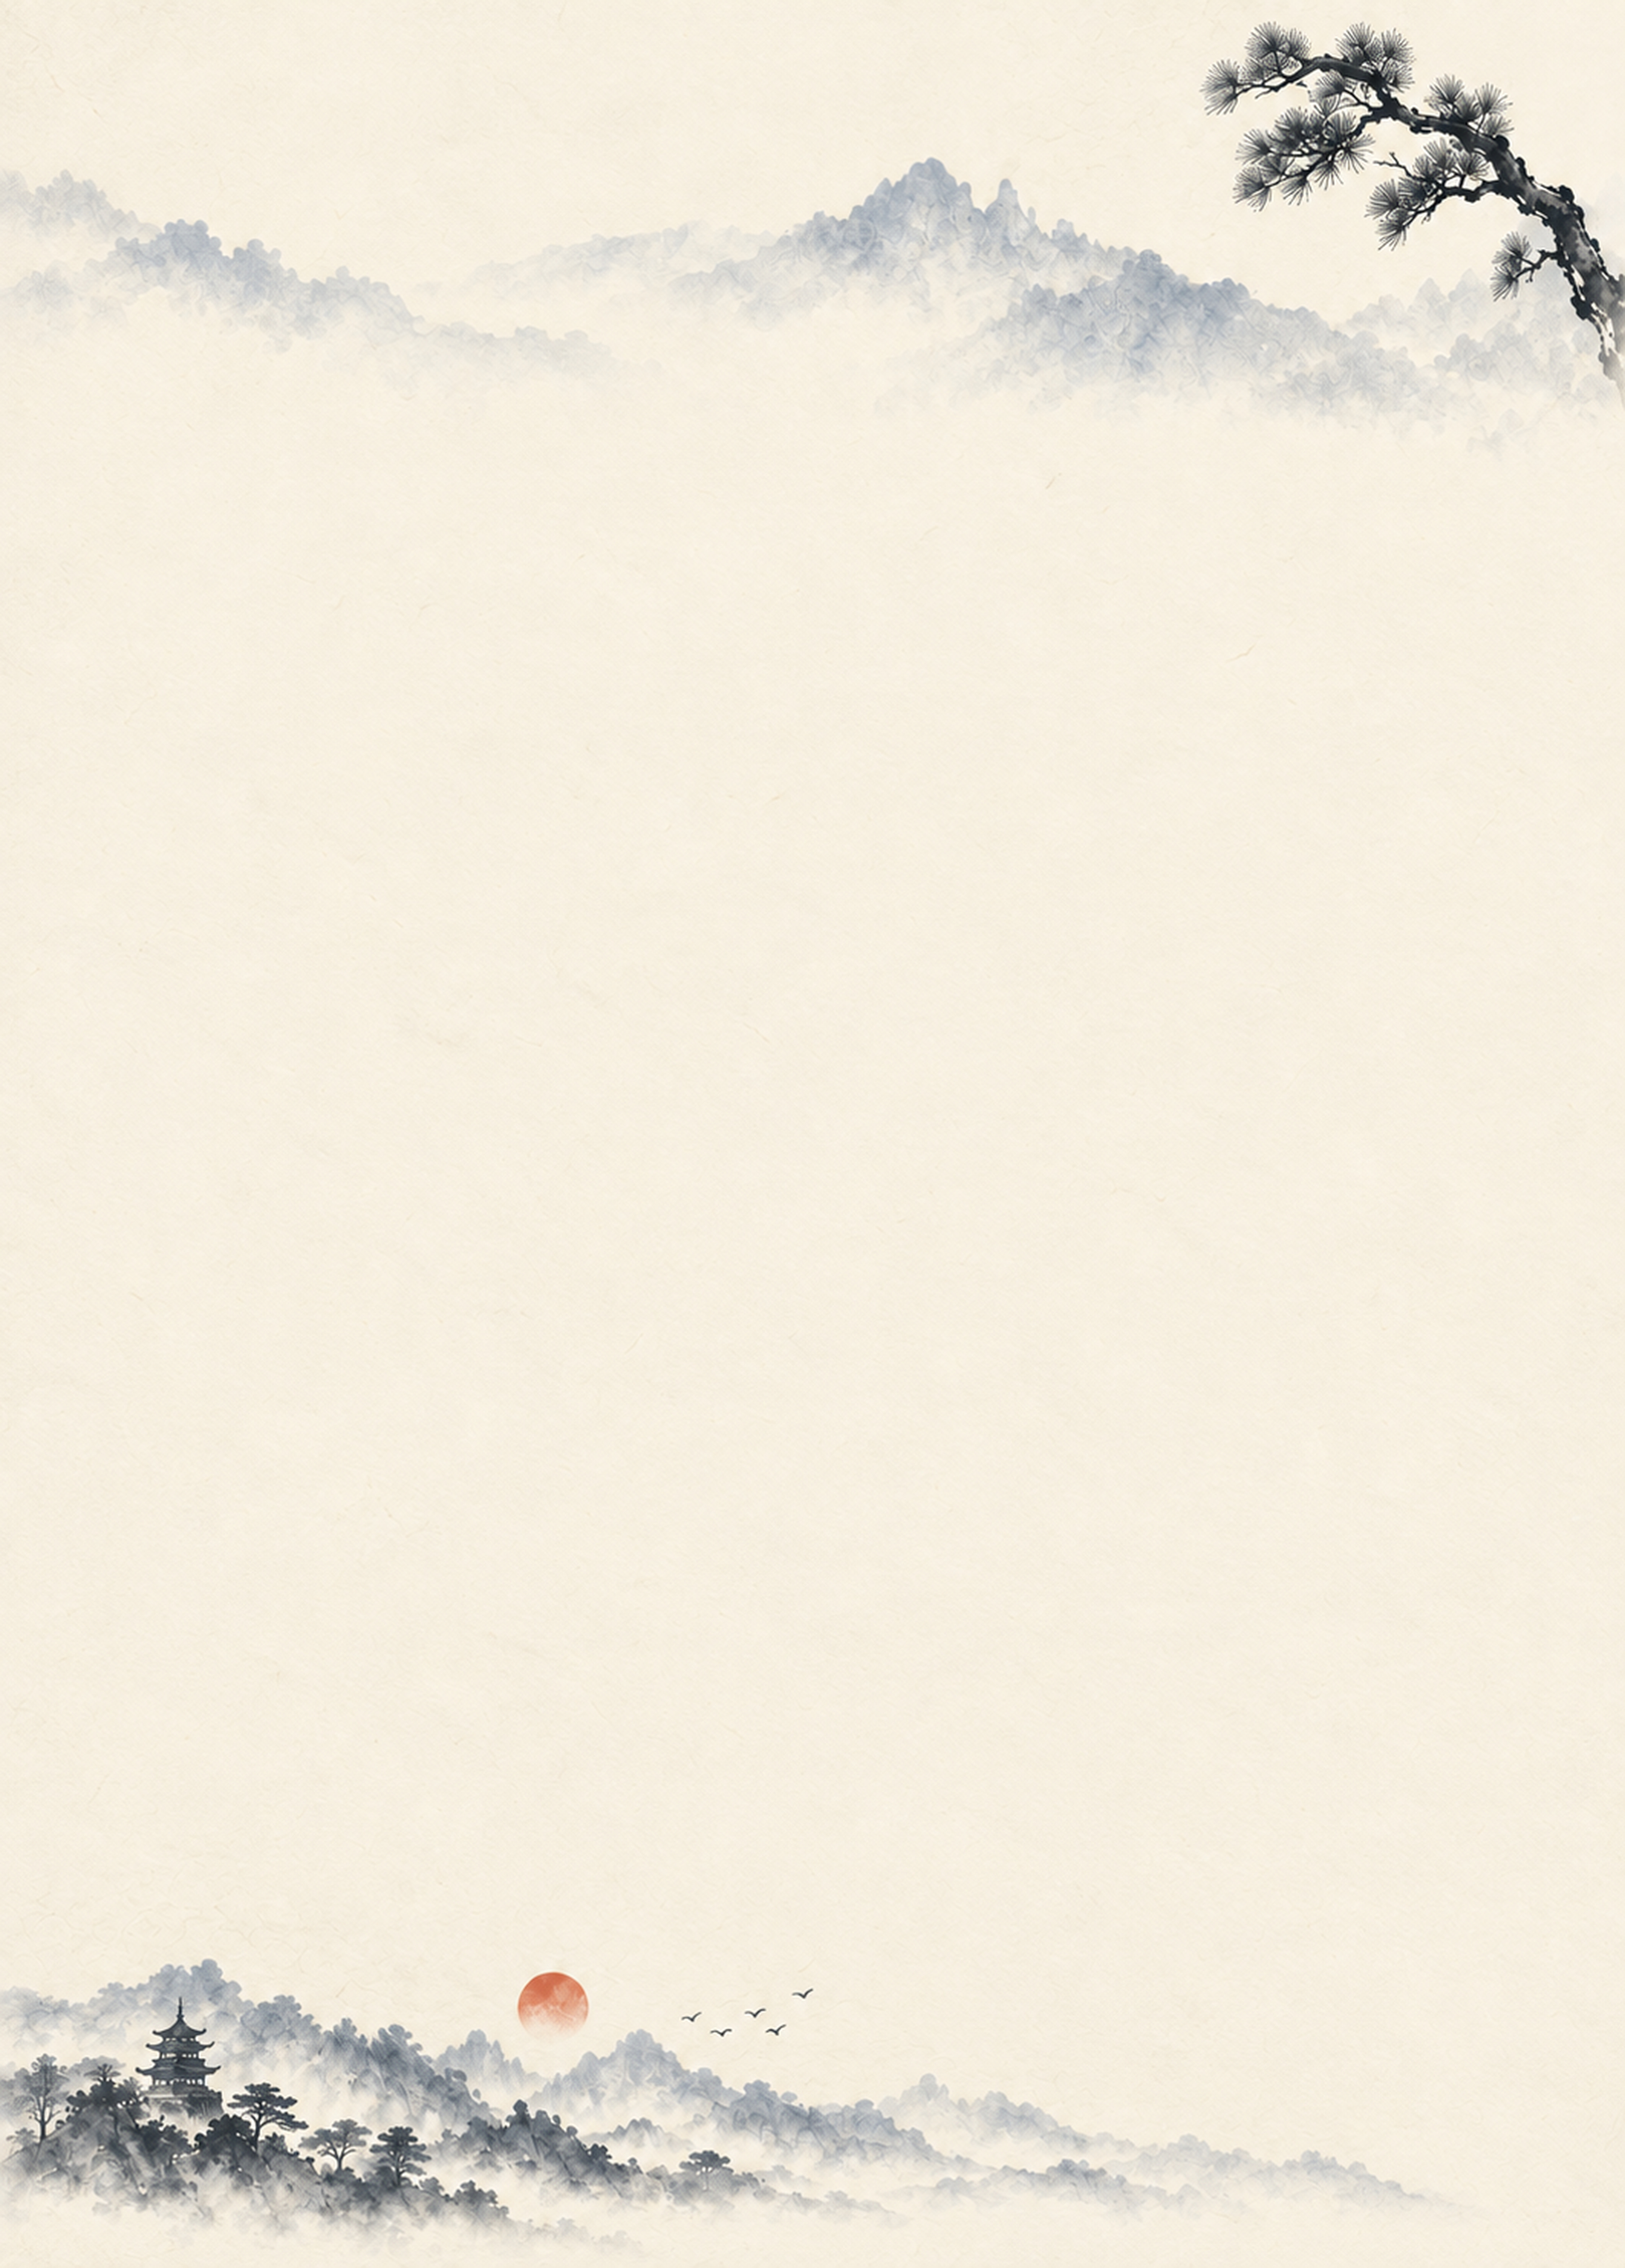
\includegraphics[width=\paperwidth,height=\paperheight]{themes/japanese-garden/assets/background-print.jpg}};
    \draw[GardenRule,line width=0.65pt]
      ([yshift=-10.0cm]current page.north) --
      ([yshift=4.0cm]current page.south);
    % Keep the mark on the clear paper beside the pine, using original vector
    % paths with no rectangular backing or image-transparency soft mask.
    \node[anchor=north east,inner sep=0pt]
      at ([xshift=-16.5cm,yshift=-1.1cm]current page.north east)
      {
\includegraphics[width=8.0cm]{themes/japanese-garden/assets/logos/lamarr.pdf}};
    % Vector QR modules leave the paper visible between them. This open area
    % has a full quiet zone and stays clear of both body text and footer logos.
    \node[anchor=south east,inner sep=0pt,align=center,text=GardenInk]
      at ([xshift=-3.5cm,yshift=4.5cm]current page.south east) {%
        \begin{minipage}{5cm}
          \centering\color{GardenInk}
          \qrcode[height=3.6cm,level=M]{https://arxiv.org/abs/2602.15146}\par
          \vspace{0.45cm}
          {\small Scan for paper}
        \end{minipage}};
  \end{tikzpicture}%
}

% ====================
% Header
% ====================

\setbeamertemplate{headline}{%
  \vskip0.75cm
  \leavevmode
  \hbox to \paperwidth{%
    \hspace*{2.2cm}%
    \begin{minipage}[t]{41cm}
      \raggedright
      {\usebeamerfont{headline title}\usebeamercolor[fg]{headline title}\inserttitle\par}
      \vspace{0.35cm}
      {\usebeamerfont{headline author}\usebeamercolor[fg]{headline author}\insertauthor\par}
      \vspace{0.15cm}
      {\usebeamerfont{headline institute}\usebeamercolor[fg]{headline institute}\insertinstitute\par}
    \end{minipage}%
    \hfill
    \begin{minipage}[t]{9.4cm}\vspace*{0pt}\end{minipage}%
    \hspace*{1.4cm}%
  }
  \vspace{0.20cm}
}

% ====================
% Ink-brush section components
% ====================

\newcommand{\gardenenso}{%
  
\begin{tikzpicture}[baseline=-0.28ex,x=1cm,y=1cm]
    \draw[GardenInk,line width=2.7pt,line cap=round]
      (0.75,0.23) arc[start angle=-18,end angle=286,radius=0.43];
    \draw[GardenRule,line width=0.65pt,line cap=round]
      (0.68,0.20) arc[start angle=-24,end angle=272,radius=0.36];
  \end{tikzpicture}%
}

\newcommand{\gardenheading}[1]{%
  \gardenenso\hspace{0.22cm}%
  {\usebeamerfont{block title}\usebeamercolor[fg]{block title}#1}%
}

\setbeamertemplate{block begin}{%
  \vskip0.15ex
  \begin{beamercolorbox}[wd=\linewidth,sep=0pt,left]{block title}
    \gardenheading{\insertblocktitle}
  \end{beamercolorbox}
  \vskip-0.45ex
  \begin{beamercolorbox}[wd=\linewidth,ht=0.055cm,dp=0cm]{block separator}\end{beamercolorbox}
  \vskip0.25ex
  \begin{beamercolorbox}[wd=\linewidth,colsep*=0ex]{block body}
    \justifying
    \setlength{\parskip}{0.6ex}
    \vskip-0.25ex
}

\setbeamertemplate{block end}{%
  \end{beamercolorbox}
  \vspace{0.45ex}
}

\setbeamertemplate{block alerted begin}{%
  \vskip0.15ex
  \begin{beamercolorbox}[wd=\linewidth,sep=0pt,left]{block alerted title}
    \gardenheading{\insertblocktitle}
  \end{beamercolorbox}
  \vskip-0.45ex
  \begin{beamercolorbox}[wd=\linewidth,ht=0.055cm,dp=0cm]{block alerted separator}\end{beamercolorbox}
  \vskip0.3ex
  \begin{beamercolorbox}[wd=\linewidth,colsep*=0.65ex,rounded=true]{block alerted body}
    \justifying
    \setlength{\parskip}{0.6ex}
    \vskip-0.3ex
}

\setbeamertemplate{block alerted end}{%
  \vskip0.25ex
  \end{beamercolorbox}
  \vspace{0.5ex}
}

\setbeamertemplate{itemize item}{\raise0.25ex\hbox{\color{GardenBlue}$\bullet$}}
\setbeamertemplate{itemize subitem}{\raise0.2ex\hbox{\color{GardenBlue}$\circ$}}
\setbeamertemplate{caption label separator}[period]

\renewcommand{\PosterFeatureBegin}[1]{\begin{block}{#1}}
\renewcommand{\PosterFeatureEnd}{\end{block}}
\renewcommand{\PosterTakeawaysBegin}[1]{\begin{alertblock}{#1}}
\renewcommand{\PosterTakeawaysEnd}{\end{alertblock}}
\renewcommand{\posteroptionalheading}[1]{%
  \begin{beamercolorbox}[wd=\linewidth,sep=0pt,left]{block title}
    \gardenheading{#1}
  \end{beamercolorbox}
  \vskip-0.45ex
  \begin{beamercolorbox}[wd=\linewidth,ht=0.055cm,dp=0cm]{block separator}\end{beamercolorbox}
  \vspace{0.45ex}%
}

% ====================
% Footer
% ====================

\newcommand{\gardenfooterlogo}[2]{%
  \raisebox{-0.5\height}{%
    \includegraphics[height=#1]{themes/japanese-garden/assets/logos/#2.pdf}}%
}

\setbeamertemplate{footline}{%
  \begin{tikzpicture}[remember picture,overlay]
    \draw[GardenRule,line width=0.65pt]
      ([xshift=2.8cm,yshift=3.3cm]current page.south west) --
      ([xshift=-2.8cm,yshift=3.3cm]current page.south east);
    \node[inner sep=0pt,anchor=center]
      at ([yshift=1.65cm]current page.south) {%
        \hbox to \dimexpr\paperwidth-5.6cm\relax{%
          \gardenfooterlogo{1.25cm}{tu-dortmund}\hfill
          \gardenfooterlogo{1.35cm}{fraunhofer-iais}\hfill
          \gardenfooterlogo{1.35cm}{fraunhofer-iml}\hfill
          \gardenfooterlogo{2.15cm}{uni-bonn}\hfill
          \gardenfooterlogo{1.70cm}{nrw}\hfill
          \gardenfooterlogo{1.90cm}{bftr}%
        }};
  \end{tikzpicture}%
  \vbox to 3.4cm{\vfil}%
}
